\chapter{Reproducibility and Artifacts}\label{app:repro}
\section{Experiment identity}
The main results come from local project artifacts \parencite{projectdata}. Training run: \texttt{20261105T022305\_489044Z}. Evaluation root: \texttt{20261105T081629\_168420Z}. The experiment source fingerprint, using ordered relative Python paths and LF-normalized file bytes, is
\begin{quote}\small\ttfamily
e27217395c51bdde1b11697346c61b5e5\allowbreak ea5a16e159b46739ebe0317d3d758f1.
\end{quote}
The selected \texttt{best\_candidate.zip} and \texttt{validated\_model.zip} are identical. Their SHA-256 is
\begin{quote}\small\ttfamily
0b58672c4e2d794b19e04e02ef9c4c56\allowbreak ab091c087481f23aa9d7b45f1d23bd1a.
\end{quote}
The final model SHA-256 is
\begin{quote}\small\ttfamily
ae7a2a0049fb52dbafc69a7d99184964\allowbreak 42694bd0fd4d1cce843fd426c12a590c.
\end{quote}
Hashes were verified unchanged after inference. The selected model has 630,000 recorded transitions and the final model 670,000. Both are in the full-distribution curriculum stage.

\section{Recorded dependencies}
\begin{table}[htbp]\centering
\caption{Versions recorded in the training manifest.}\label{tab:versions}
\begin{tabular}{ll}\toprule Component & Version\\\midrule
Python & 3.14.3\\NumPy / SciPy & 2.5.3 / 1.18.0\\
PyTorch & 2.14.1+cu126\\Gymnasium & 1.3.0\\
Stable-Baselines3 & 2.9.0\\PyBullet & 3.2.7\\
gym-pybullet-drones & 2.2.0\\CVXPY & 1.9.3\\
CLARABEL / SCS & 0.11.1 / 3.3.1\\
Matplotlib & 3.11.2\\\bottomrule
\end{tabular}\end{table}
These are recorded environment versions, not a claim that every later library version reproduces identical trajectories. The report does not infer hardware speed from these package versions.

\section{Evaluation commands}
The following command evaluates the selected checkpoint and creates a new dated output directory. It does not train a policy.
\begin{lstlisting}[language={},caption={Evaluate the selected policy on all three scenarios.}]
python evaluate.py --model results/training/20261105T022305_489044Z/validated_model.zip --case all
\end{lstlisting}
For the final-policy comparison, replace the filename by \texttt{ppo\_final.zip}. The saved evaluation runner in the review directory performs the sixty-goal tests and blocks learning calls. It uses the stored coordinates and seeds to keep the checkpoint comparison paired. A rerun should use a new output directory rather than overwrite prior evidence.

\section{Figure inventory}
The main external figure files are listed below. Every trajectory and separation figure uses the selected 630,000-step checkpoint. The training figure covers the whole run; the additional-goal figure explicitly compares both checkpoints. A machine-readable \texttt{figure\_sources.json} is included in the Overleaf package.

\begin{longtable}{p{.44\textwidth}p{.49\textwidth}}
\caption{Figure files and their role.}\label{tab:figures}\\
\toprule File in \texttt{figures/} & Purpose\\\midrule\endfirsthead
\toprule File & Purpose\\\midrule\endhead
\texttt{learning\_progress.png} & Fixed and stage validation history\\
\texttt{goal\_generalization.png} & Additional goal success for 630k and 670k\\
\texttt{selected\_comparison.png} & Main arrival and separation comparison\\
\texttt{selected\_goal\_errors.png} & Goal-error curves for the selected policy\\
\texttt{case1\_trajectory.png} & Linear-obstacle 3D trajectories\\
\texttt{case2\_trajectory.png} & Accelerating-obstacle 3D trajectories\\
\texttt{case3\_trajectory.png} & Figure-eight 3D trajectories\\
\texttt{case3\_separation.png} & Figure-eight time-aligned safety evidence\\
\texttt{case1\_separation.png} & Supplementary linear-case distance history\\
\texttt{case2\_separation.png} & Supplementary accelerating-case distance history\\\bottomrule
\end{longtable}

\begin{figure}[htbp]\centering
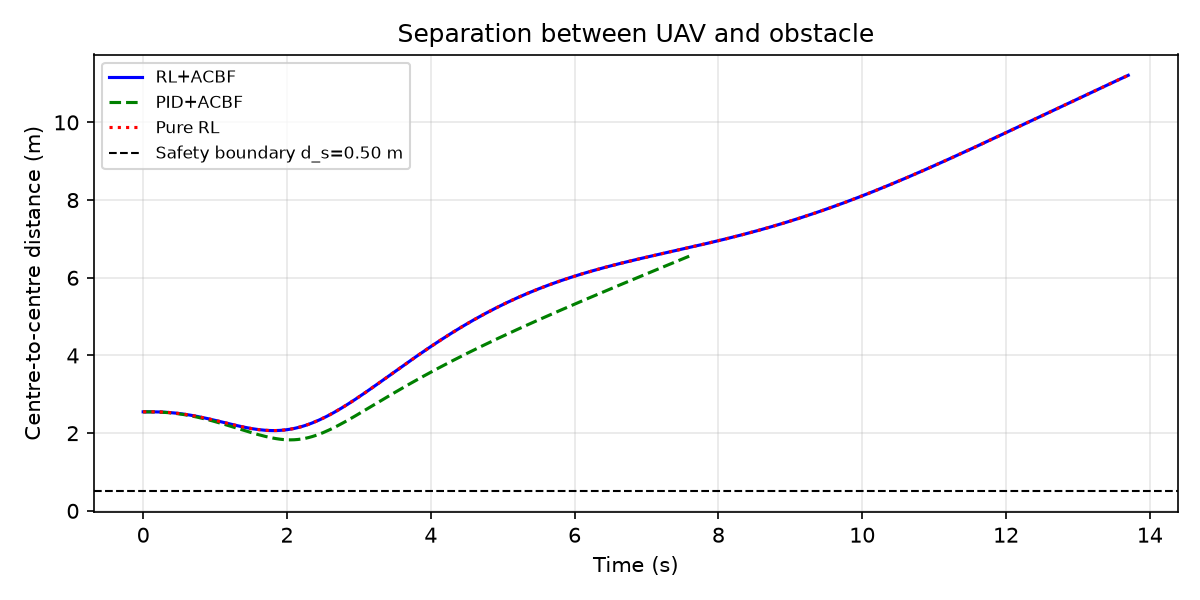
\includegraphics[width=.92\textwidth]{case1_separation.png}
\caption{Supplementary case 1 separation history for the selected checkpoint.}\label{fig:separation1}
\end{figure}
\begin{figure}[htbp]\centering
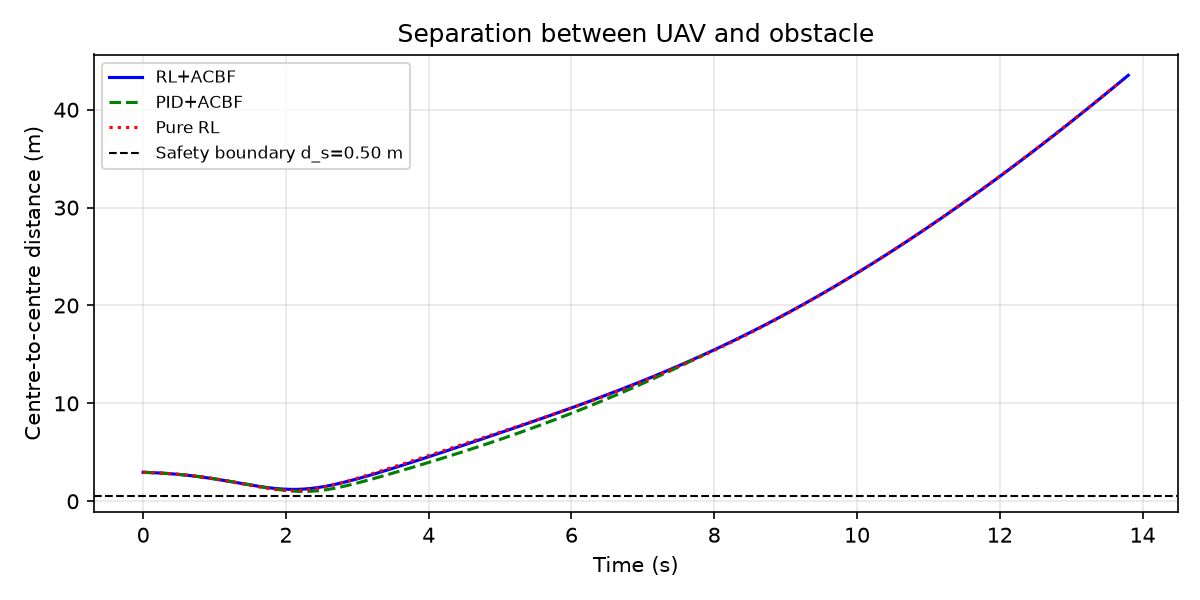
\includegraphics[width=.92\textwidth]{case2_separation.png}
\caption{Supplementary case 2 separation history for the selected checkpoint.}\label{fig:separation2}
\end{figure}

\section{Interpretation checklist}
An arrival claim must use both position and speed/hold conditions. A safety claim must distinguish the 0.50~m buffer from the 0.40~m collision threshold. A checkpoint comparison must identify the actual weights used. A generalization claim must identify which goals and training seeds were tested. A real-time claim requires wall-clock deadline measurements. These distinctions are necessary to reproduce the conclusions of this report without overstating the evidence.
